\begin{figure}[tb]
    \centering
    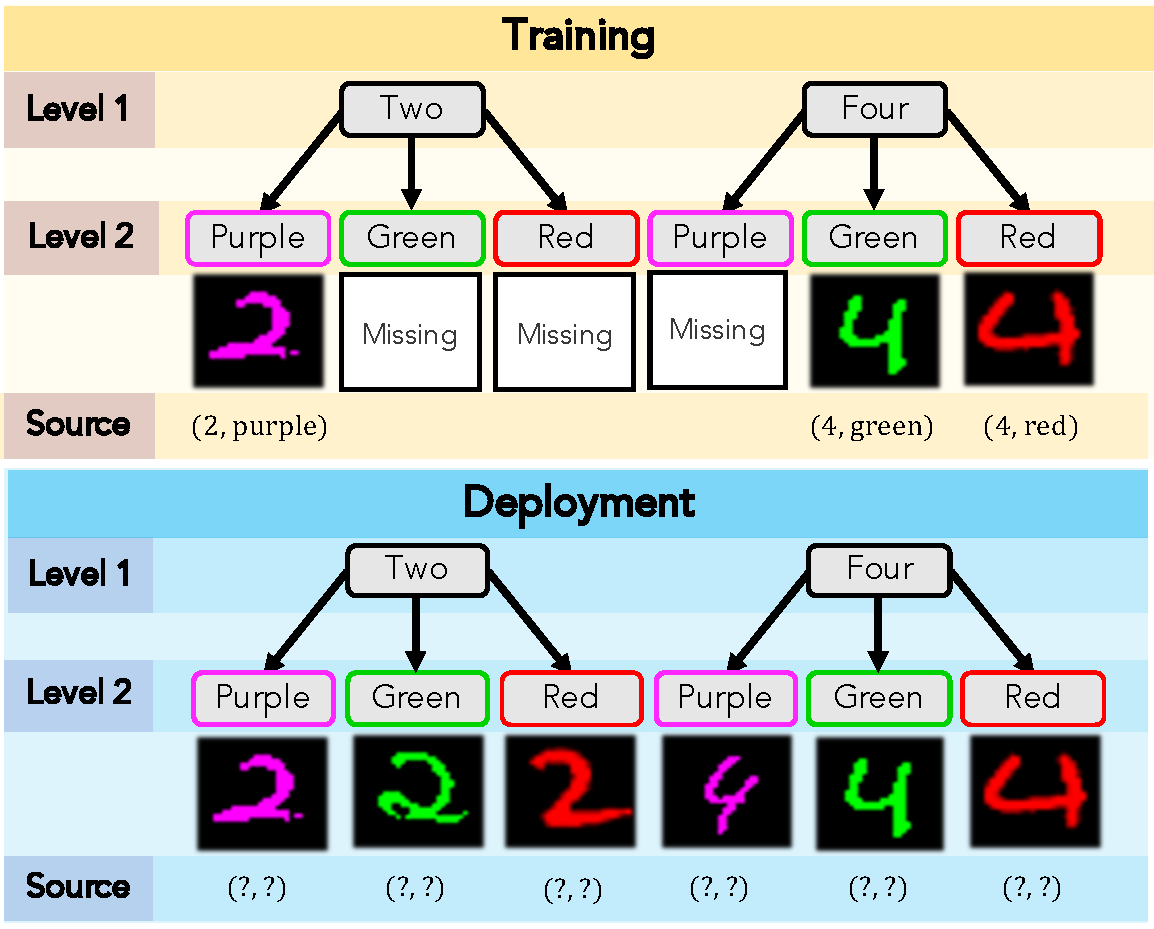
\includegraphics[width=0.7\columnwidth]{supmatch/figures/illustrations/problem_setup.pdf}
    \caption{%
      Illustration of our general problem setup. 
      %
      We assume the data follows a two-level hierarchy in which the first level corresponds to the class-level information (digit) and the second level corresponds to subgroup-level information (color).
      %
      While all digits appear in the training set (Top), not all digit-color combinations (sources) do; these gaps in conditional support give rise to a spurious correlation between digit and color, where the former is completely determined by the latter in the training set (giving the mappings $\textrm{{\color{purple}purple}} \rightarrow \texttt{2}$ and $\textrm{{\color{green}green}} \lor \textrm{{\color{red}red}} \rightarrow \texttt{4}$ as degenerate solutions to the classification problem), yet this same correlation does not hold for the deployment set (Bottom) which contains samples from the missing combinations.
      %
      To disentangle the (spurious) subgroup- and class-related information, we make use of an additional dataset that is representative of the data the model is expected to encounter at deployment time, in terms of the sources present.
    }%
    \label{fig:problem-setup}
\end{figure}
